\providecommand{\rasd}{..}
\documentclass[../RASD.tex]{subfiles}

\begin{document}

    \chapter{Specific requirements}\label{ch:specific-requirements}
    This section contains all of the functional and quality requirements of the system. It gives a detailed description of the system and all its features.
        \section{External interface requirements}\label{sec:external-interface-requirements}
            \subsection{User Interfaces}\label{subsec:user-interfaces}
            \subsection{Hardware Interfaces}\label{subsec:hardware-interfaces}
        The system has no hardware interface, because SafeStreet does not interact physically with other systems.
            \subsection{Software Interfaces}\label{subsec:software-interfaces}
            The system uses an API provided by the municipality that allows SS to cross incidents received with its database in order to suggest possible interventions on the high-risk areas. Moreover, the system uses third party API in order to display the map of the city and decode license plates from images (in order to blur them from citizens).
            \subsection{Communication Interfaces}\label{subsec:communication-interface}
            SafeStreet uses secure internet connection in order to provide a reliable exchange of messages between clients and server, like HTTPS.
        \section{Functional requirements}\label{sec:functional-requirements}
            \subsection{Scenarios}\label{subsec:scenarios}
                \textbf{Scenario 1:} Federico is a citizen who wants to report a parking violation. For this purpose, he decides to use SafeStreet. He downloads the application on his smartphone and proceeds to sign up. He is asked to insert an email and a password, and of course, being only a citizen, the authority ID is not required by the system. Federico inserts his personal email and his password, but the system tells him that the given password is shorter than 8 characters, so he tries again with a new one. Eventually he is able to insert a valid password, accepts the Terms and conditions and taps on “Create an Account”. He is now successfully signed up, after receiving a confirmation email by SafeStreet. He tries to login to the application by inserting the same email and password originally submitted. The system accepts the credentials and Federico is in. Now, he navigates to the report section, where he is asked to insert one or more images and select the type of violation, and optionally write a note. Federico takes and insert 2 photos, one of them also containing the license plate of the vehicle, so that the police can fine the transgressor. Once done, Federico can also see his report, through the map section.
    \newline
    \newline
                \textbf{Scenario 2:} Evandro is a police officer whose job is to fine cars that committed violations in the city of Milan. For that purpose, he decides to use SafeStreet. He downloads the app and signs up using his work email, a strong password of 10 characters, and he inserts his ID to the system. He is now recognized as an authority and can use all the complete functionalities of SS and has access to all the sensitive information, like the license plates uploaded by users. Once in, Evandro navigates to the map section and selects one of the violations displayed in the map, but that violation, even if it breaks the law, does not contain an image with the license plate visible, so Evandro cannot fine the transgressor.
    \newline
    \newline
                \textbf{Scenario 3:} Erik is a police officer whose job is to fine cars that committed violations in the city of Milan. For that purpose, he decides to use SafeStreet. He downloads the app and signs up using his work email, a strong password of 10 characters, and he inserts his ID to the system. He is now recognized as an authority and can use all the complete functionalities of SS and has access to all the sensitive information, like the license plates uploaded by users. Once in, Erik navigates to the map section and selects one of the violations displayed in the map. That violation contains an image with the license plate of the transgressor. After having judged the report, he decides to fine him using a third-party system. After that, Erik marks the report as “fined”, so that SafeStreet can then build statistics.
    \newline
    \newline
                \textbf{Scenario 4:} Baldo is a police officer that has on the smartphone SS and is already logged in.

                                    During his work detail, Baldo goes in the extra area for the municipality. Baldo sees on the map of SS that there are some violation in the neighborhood under Baldo’s custody. So Baldo opens one of the violations and he discovers that it’s a “parking in the wrong way”. Baldo wants to check the gravity of the violation so he looks carefully at the three photos of the violation, Baldo analyzes them and decides to not generate a traffic tickets because even if the report underlines a borderline situation, the car respects all the laws.

                                     So Baldo doesn’t mark as “fined” the report because he doesn’t generate a traffic ticket for that.
    \newline
    \newline
                \textbf{Scenario 5:} Tom is an old man who has downloaded SS on his smartphone.

                Tom wants to bike to the market, but he feels unsafe because people usually park their cars on the bicycle lane, so he decides to check on SafeStreet if any violation has been reported on the way to the market.  Looking on the map, he saw a violation classified as “parking on bicycle line” and opens it to see the time of the report. When he opens the dossier, he takes a look at the picture and notices that the car is just close to the bike lane, but it does not really obstruct the passage. Tom thinks that the car is parked correctly and does not represent a violation, so he opens the feedback area and sends a negative feedback, selecting the option “false violation”.
                \newline
                \newline
                \textbf{Scenario 6:} Tom from scenario S5, during breakfast checks also another violation always on the way to his work.

                 He opens the report on the map and analyzes the photos. The report is marked as “trash can on bike line” but on the pictures there are only a car parked on zebra crossing. In this case the description doesn’t match with the images and Eddy one more time goes in the report area of the violations and sends a negative feedback to SS pushing on “negative feedback” button.

                SS uses this feedback to build statistics
    \newline
    \newline
                \textbf{Scenario 7:} The municipality of Monza wants to improve its management of the traffic violations. In order to do that, they decide to be supported by SafeStreet as an immediate and low-cost solution. They offer a public database on which all the accidents in the territory are registered, to allow SafeStreet to collect data.

                After only two weeks SafeStreet provide the first report to Monza’s municipality: the application notice that just a few meters away from a reported accident three no parking zone violations have been reported, so it sends a notification to the municipality to suggest to add some anti-parking poles.
    \newline
    \newline
                \textbf{Scenario 8:} Mary is a young woman who lives in Milan and has a six year-old son. She must enrol his son to the elementary school and she has already found two possible options, but since they are both located in an intense traffic area she is afraid that they could be dangerous. The municipality of Milan provides through SafeStreet the information about all the accidents occurring on its territory, so Mary wants to use this information to take a decision.
                She queries the system to get all the possible unsafe areas of Milan. She finds out that her first option is located in a high-level dangerous zone: clicking on the area, she notices that three car accidents occurred at a crossroad that is located just few meters from the school building. Since her second option is in an area not marked as dangerous by SafeStreet, and where no accidents have been reported, Mary decides that she will enrol her son there.

            \subsection{Use Case Diagrams}\label{subsec:Use-case-diagrams}
                    \begin{figure}[H]
                        \centering
                        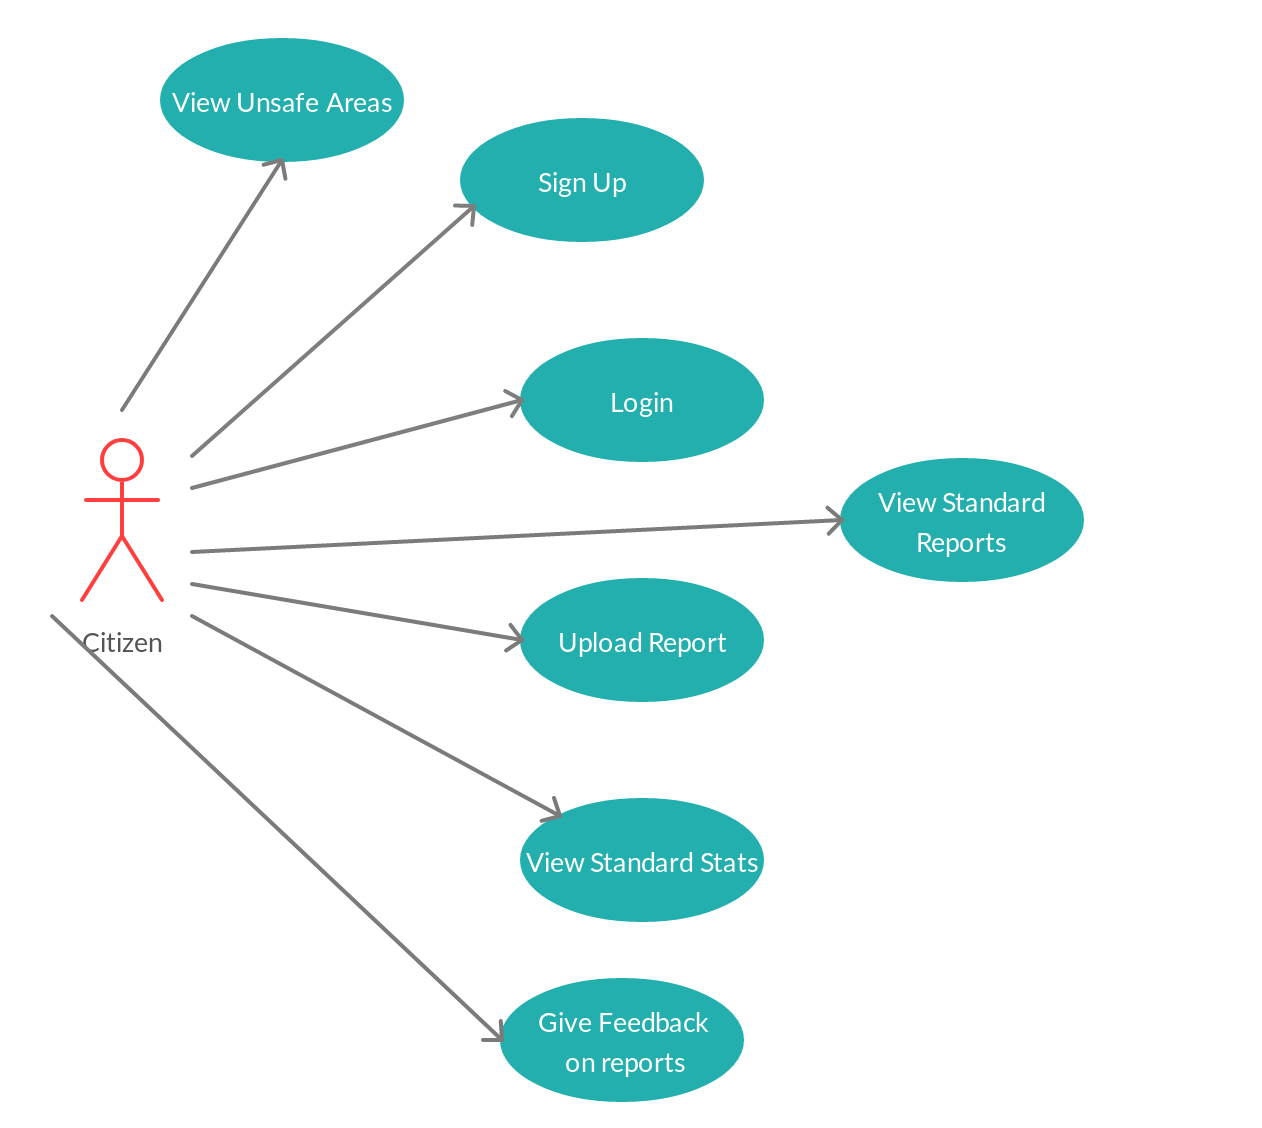
\includegraphics[scale = 1]{assets/citizenUC.png}\\[1.6 cm]
                        \caption[Citizen \textit{Use Case Diagram}]{Citizen \textit{Use Case Diagram}}
                    \end{figure}
                    \begin{figure}[H]
                        \centering
                        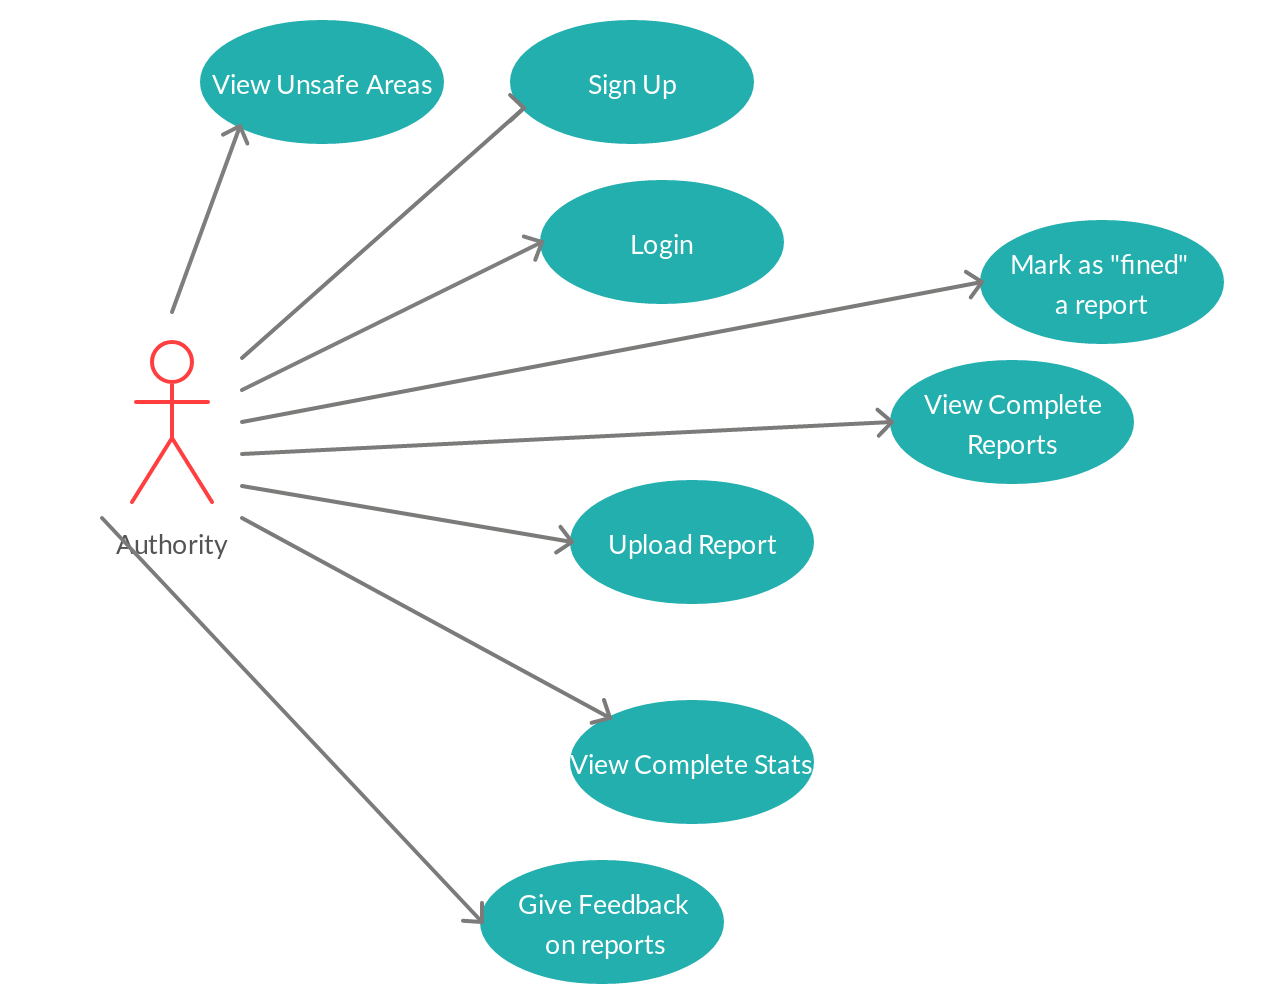
\includegraphics[scale = 1]{assets/authorityUC.png}\\[1.6 cm]
                        \caption[Authority \textit{Use Case Diagram}]{Authority \textit{Use Case Diagram}}
                    \end{figure}
                    \begin{figure}[H]
                        \centering
                        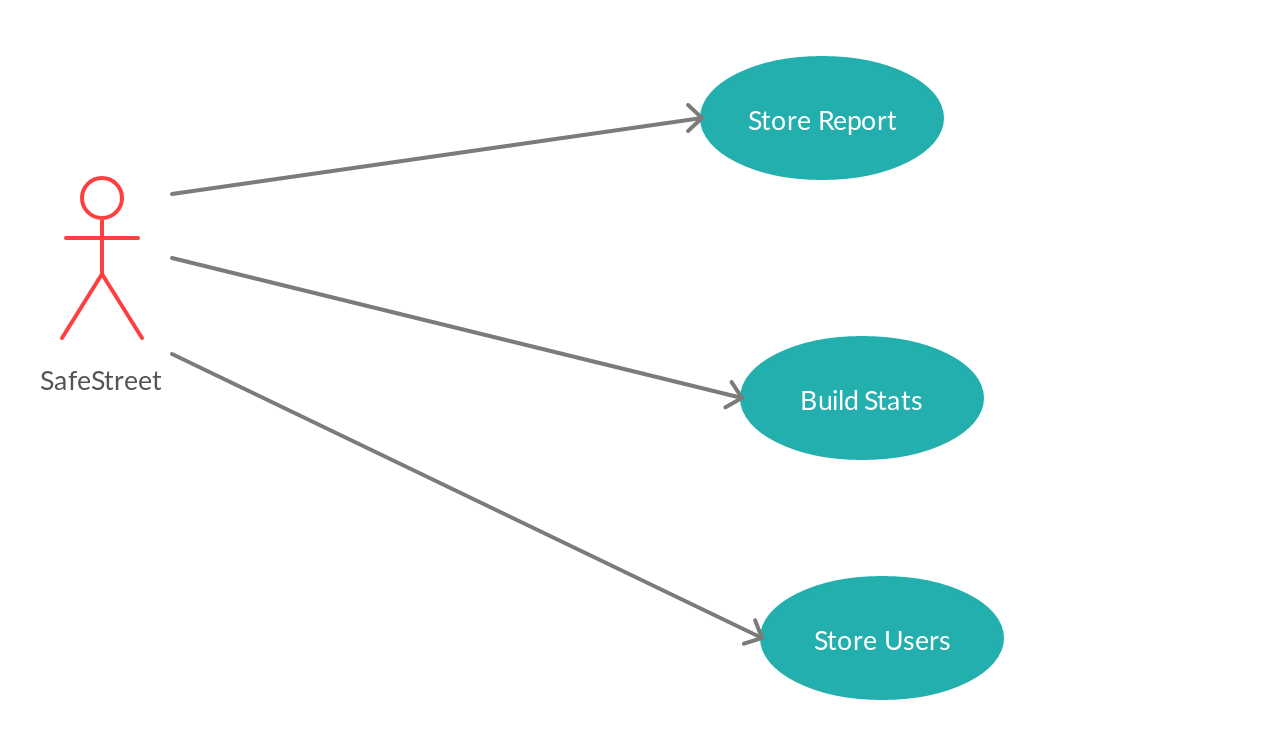
\includegraphics[scale = 1]{assets/safeStreetUC.png}\\[1.6 cm]
                        \caption[SafeStreet \textit{Use Case Diagram}]{SafeSteet \textit{Use Case Diagram}}
                    \end{figure}
                    \newpage
            \subsection{Use Case Analysis}\label{subsec:use-case-analysis}
                \subfile{specific_requirements/functional_requirements/use_case_analysis/use_case_analysis.tex}
            \newpage
            \subsection{Sequence Diagrams}\label{subsec:sequence-diagrams}
                \begin{figure}[H]
                    \centering
                    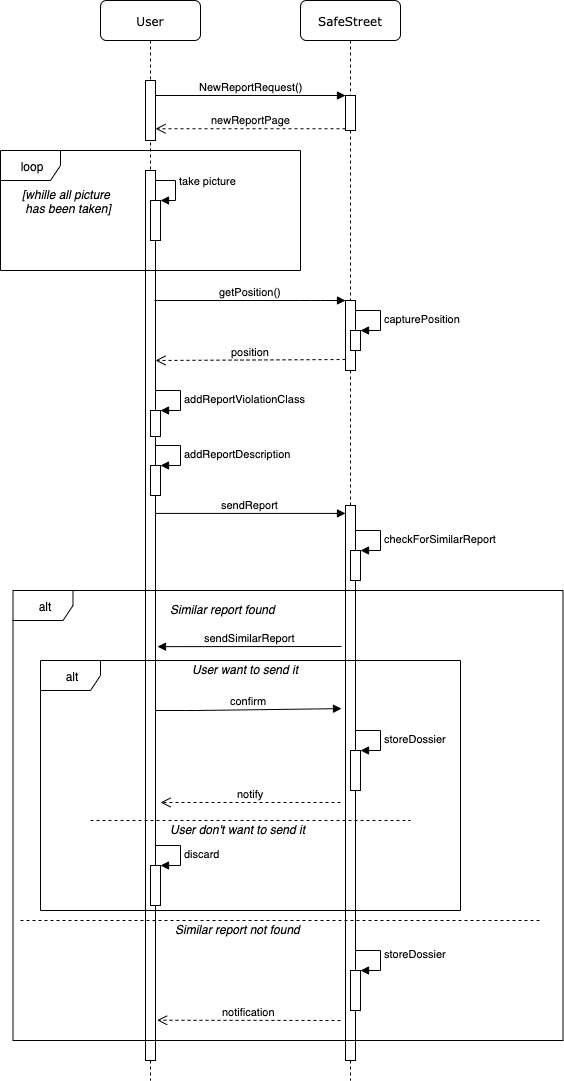
\includegraphics[scale = 2]{assets/sendReportSD.png}\\[1.6 cm]
                    \caption[Send Report \textit{Sequence Diagram}]{Send Report \textit{Sequence Diagram}}
                \end{figure}
                \begin{figure}[H]
                    \centering
                    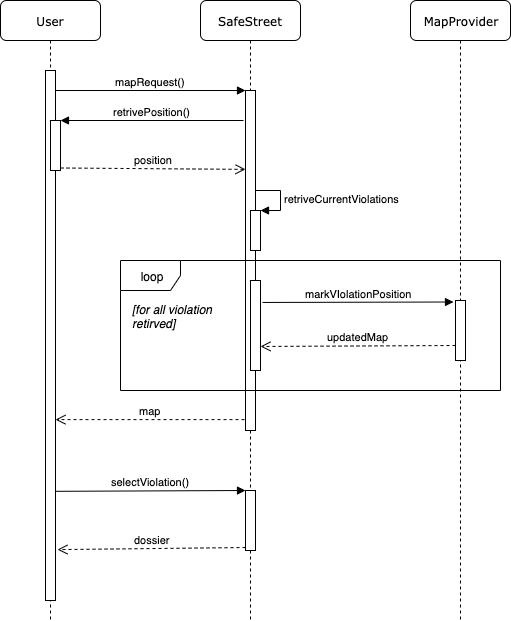
\includegraphics[scale = 2]{assets/getViolationSD.png}\\[1.6 cm]
                    \caption[Get Violations \textit{Sequence Diagram}]{Get Violations \textit{Sequence Diagram}}
                \end{figure}
                \begin{figure}[H]
                    \centering
                    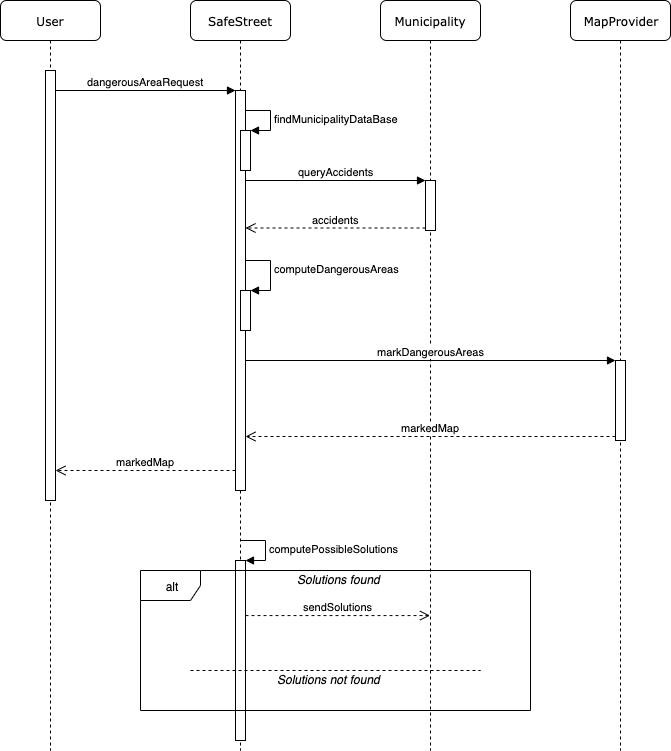
\includegraphics[scale = 2]{assets/getDangerousAreasSD.png}\\[1.6 cm]
                    \caption[Get Dangerous Areas \textit{Sequence Diagram}]{Get Dangerous Areas \textit{Sequence Diagram}}
                \end{figure}
                \begin{figure}[H]
                    \centering
                    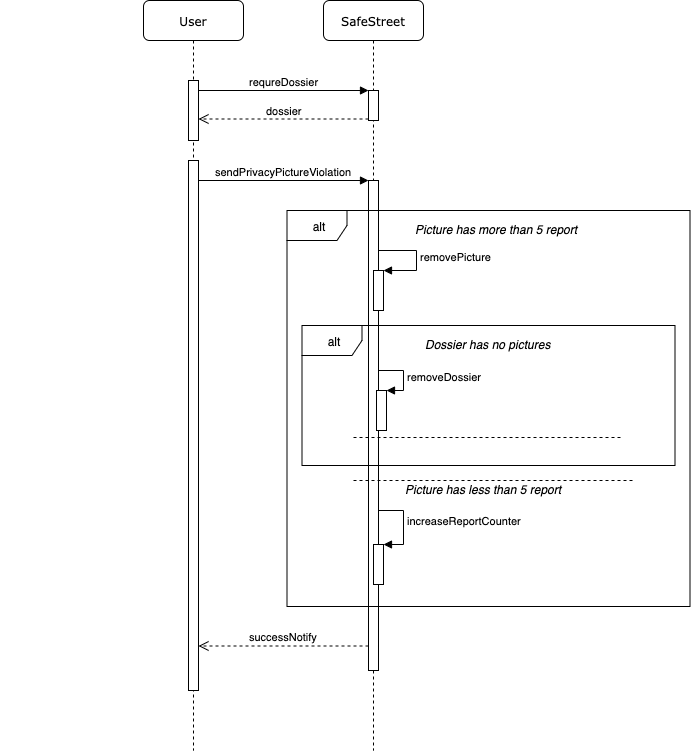
\includegraphics[scale = 2]{assets/sendFeedbackSD.png}\\[1.6 cm]
                    \caption[Send Feedback \textit{Sequence Diagram}]{Send Feedback \textit{Sequence Diagram}}
                \end{figure}
            \newpage
            \subsection{Requirements, Domain Assumptions, Goals Matrix}\label{subsec:requirements,-domain-assumptions,-goals-matrix}
                The following is a list of requirements for SafeStreet.
                \begin{enumerate}
                    \requirement{1} Unregistered user cannot use SafeStreet.
                    \requirement{2} In signing up, users must provide an email and a password.
                    \requirement{3} In signing up, an authority must also provide an ID.
                    \requirement{4} In signing up, users must accept “terms \& conditions”.
                    \requirement{5} SS identifies a user by its email.
                    \requirement{6} SS collects user data in its database.
                    \requirement{7} SS stores all reports in its database.
                    \requirement{8} SS retrieves reports from its database.
                    \requirement{9} SS authenticates a user when tries to log in.
                    \requirement{10} Users can view the reports in the map.
                    \requirement{11} Authorities can see all the sensitive information contained in a report.
                    \requirement{12} Citizens cannot see sensitive information in a report.
                    \requirement{13} Users can view unsafe areas in the map.
                    \requirement{14} Users can delete reports they submitted within a day.
                    \requirement{15} Users can edit reports they submitted within a day.
                    \requirement{16} Users can upload valid reports.
                    \requirement{17} A report must contain at least one image.
                    \requirement{18} A report must indicate the type of violation.
                    \requirement{19} A report is valid if and only if R17 and R18 are satisfied.
                    \requirement{20} Images containing sensitive information (like license plates) must be blurred by the system.
                    \requirement{21} The system must notify the user if the report submitted is not valid.
                    \requirement{22} For each type of statistics there must be at least user from which SS takes data.
                    \requirement{23} A user can access to feedback area for each report.
                    \requirement{24} A user can select negative feedback for each report.
                    \requirement{25} Authorities can see suggestions for possible interventions.
                    \requirement{26} During adding a new report, if there is a report of same type, in the same position and at the same date, SS shows the report stored to the user if the violation is the same.
                    \requirement{27} Authorities can mark a report as “fined”.
                    \requirement{28} User can query SS to achieve a specific report.
                    \requirement{29} SS retrieves incidents from municipality database.
                \end{enumerate}
                The following is an analysis, for each goal of the system to be, of the requirements R\textsubscript{n} and the domain assumptions D\textsubscript{n} that satisfy the goal itself and of these cases relative to it.
                \begin{enumerate}
                    \goal{1} The application will allow users to upload pictures of the traffic violations, including pictures, date, time, classification, and optionally a textual description.
                        \begin{itemize}
                            \requirement{} 1,2,3,4,5,6,9,14,15,16,17,18,19,20,21,26
                            \assumption{} 1,2,4
                            \item Requirements are about the correctness of the reports while the domain assumptions are about the gps position and the license plate.
                        \end{itemize}
                    \goal{2} The application will allow users to view a map of the violations registered in the last day.
                    \begin{itemize}
                        \requirement{} 1,,2,3,4,5,6,7,8,1011,12,17,18,28
                        \assumption{} 1,3
                        \item Requirements are about the correctness of the reports while the domain assumptions are about correctness of the map.
                    \end{itemize}
                    \goal{3} The application will allow users to see the violations uploaded by other users; however, citizens won’t be able to see sensitive pictures, while authorities will be allowed.
                    \begin{itemize}
                        \requirement{} 1,2,3,4,5,6,7,8,11,12,17,18,19,20
                        \assumption{} 2,3,4
                        \item Requirements are about the correctness of the reports and the different level of visibility of citizen and authority while the domain assumptions are about the correctness of the map.
                    \end{itemize}
                    \goal{4} Users will be able to query the system to get all the reported violations that correspond to some temporal, geographical or categorical parameters.
                    \begin{itemize}
                        \requirement{} 5,6,7,8,12,17,18,19,22,29
                        \assumption{} 2,4
                        \item Requirements are about the correctness of the reports and the query on the database while the domain assumptions are about the integrity of the data stored.
                    \end{itemize}
                    \goal{5} Users can give a feedback about violations uploaded by other users to SS.
                    \begin{itemize}
                        \requirement{} 1,2,3,4,5,6,7,8,23,22,24
                        \assumption{} 2,4
                        \item Requirements are about the correctness of the reports and feedback area of the user while the domain assumptions are about the the integrity of data stored.
                    \end{itemize}
                    \goal{6} If SafeStreets can get the information about accidents by the municipality, it will give the possibility to merge them with its data to identify potentially unsafe areas.
                    \begin{itemize}
                        \requirement{} 7,8,13,16,17,18,19,22,29
                        \assumption{} 3,5
                        \item Requirements are about the correctness of the reports and the capability of SS to find unsafe area while the domain assumptions are about the consistency of data on accidents.
                    \end{itemize}
                    \goal{7} If SafeStreets can get the information about accidents by the municipality, it will give the possibility to merge them with its data to suggest possible interventions.
                    \begin{itemize}
                        \requirement{} 5,6,7,8,17,18,19,20,22,25,29
                        \assumption{} 3,5
                        \item Requirements are about the correctness of the reports and capability of SS to build statistics while the domain assumptions are about the consistency of data on accidents.
                    \end{itemize}
                    \goal{8} The system will use the information about violations, accidents and fines that will collect by both users and authorities to build statistics.
                    \begin{itemize}
                        \requirement{} 5,6,7,8,17,18,19,23,24,22,27,29
                        \assumption{} 2,5
                        \item Requirements are about the correctness of the reports and capability of SS to build ststistics while the domain assumptions are about consistency of data on accidents.
                    \end{itemize}\end{enumerate}
                \newpage
                \textbf{Traceability matrix:}
                %%%%%%%%%
                \begin{center}
                    \begin{tabular}{ ||c||c|| }

                        \hline
                        \textbf{Use case} & \textbf{Requirements}  \\ \hline
                        [\textbf{1}] Citizen signs up & 1,2,4,5,6 \\ \hline
                        [\textbf{2}] Authority signs up & 1,2,3,4,5,6\\ \hline
                        [\textbf{3}] User signs in & 1,5,9\\ \hline
                        [\textbf{4}] User reports a violation & 7,16,17,18,19,20,21,22\\ \hline
                        [\textbf{5}] Feedback by a User & 7,10,11,12,20,23,24\\ \hline
                        [\textbf{6}] Mark a report as “fined” & 7,11,12,17,18,19,20,27\\ \hline
                        [\textbf{7}] Violation query by a user & 7,8,17,18,19,20,28\\ \hline
                        [\textbf{8}] Display violation on the map & 7,8,10,11,12,,17,18,19\\ \hline
                        [\textbf{9}] View unsafe areas & 7,8,11,12,13,29\\ \hline
                        [\textbf{10}] View statistics on crime & 7,8,11,12,20,22\\ \hline
                        [\textbf{11}] View statistics on SS & 7,8,11,12,20,22\\ \hline
                        [\textbf{12}] User edits a report & 7,8,15,16,17,18,19,21\\ \hline
                        [\textbf{13}] User removes a report & 7,8,14,16,17,18,19,21\\ \hline
                        [\textbf{14}] User reports something that is already stored & 7,16,17,18,19,20,21,26\\ \hline
                    \end{tabular}
                \end{center}
                %%%%%%%%%
        \section{Performance requirements}\label{sec:performance-requirements}
        The system must be able to serve a great number of users at the same time. It must guarantee that the query of the system by a user will provide the history of the violation in a short time, even with a big amount of report. For every image uploaded for a report, the system must allow a file dimension of at list 5 Mb. In the map representation of the violation, the position of a report must be no more than 10 meters away from the actual position indicated.
        \section{Design constraints}\label{sec:design-constraints}
            \subsection{Standard compliance}\label{subsec:standard-compliance}
            Since the system will show to the user pictures taken by other people, the application refers to the European General Data Protection Regulation (GDPR) as regards the privacy protection. That means that no licence plate will be show to the users if they have not an authority level account.
            \subsection{Hardware limitations}\label{subsec:hardware-limitations}
            The application works independently of the hardware on which is running. However, the availability of some functionality will be dependent on the device used and its components.

            Internet connection will be required to use the application, since all the functionality are based on it.

            It will be possible to upload a report only if the device is provided by a camera, since the violation's photographs will must be taken within the context of the application, and will not be possible to upload a saved picture. The GPS will be needed to enable geolocation to automatically set the position of a report or of the violation map.
            \subsection{Any other constraints}\label{subsec:any-other-constraints}
        \section{Software system attributes}\label{sec:software-system-attributes}
            \subsection{Reliability}\label{subsec:reliability}
            The system must run continuously without interruption. Since the application require to the user to take and send the pictures in real time, the operation of uploading a report is the most critical and is required to work without roll back, because it could be no more possible for the user to retake them. For this situation, the system must also give the possibility to re-upload the same picture taken if something goes wrong while sending them to the server.

            The system has to guarantee the data integrity as much as possible, for example by duplicating the database used to store violations. If the availability of date couldn’t be provided anyway (for example, because of missing internet connection or server connection error) the application must notify the user throw an alert.
            \subsection{Availability}\label{subsec:availability}
            Since the application work in real time for the upload of a violation, the system must reduce the unavailability as much as possible. The error management systems described before must be projected to expect SafeStreet to be available 99.5 \% of the time.
                    \subsection{Security}\label{subsec:security}
            The data provided by the users to join the application (email, password, and eventually an ID) are sensitive information and must be protected. SafeStreet must never provide that information in any way to any person. To prevent information stealing, an encryption technique must be used while exchanging data with a user. Moreover, all necessary measures to avoid external or internal attacks to the data bases must be taken.
            \subsection{Maintainability}\label{subsec:maintainability}
            The developing of the application must be such to allow future modification or fixing. The system could be expanded with new features in the future, so the software must be also suitable to new functionalities. To reach those goals, the software must be well commented, readable and use appropriate design patterns.
            \subsection{Portability}\label{subsec:portability}
            The application main functionality work in real time and outdoors, so it will be required that the application will be able to work on smartphones. Moreover, since it must be used by many different people, it will must be suitable to all the most important mobile operative systems.

            To be able to reach more people, SafeStreet will have to be compatible to as many devices and technologies as possible.

\end{document}
